% Data-abstraction barriers in the rational-number package, used in Section 2.1.2.
%
% Drawn rather than vendored because two of the labels differ: what the
% original names cons, car and cdr is written (n, d) and x[0] here, and the
% layer beneath is the tuple rather than a pair of unspecified provenance.
%
% The shape is upstream's: a stack of named boxes, each straddling a rule that
% runs the width of the figure, with the thing being abstracted named between.

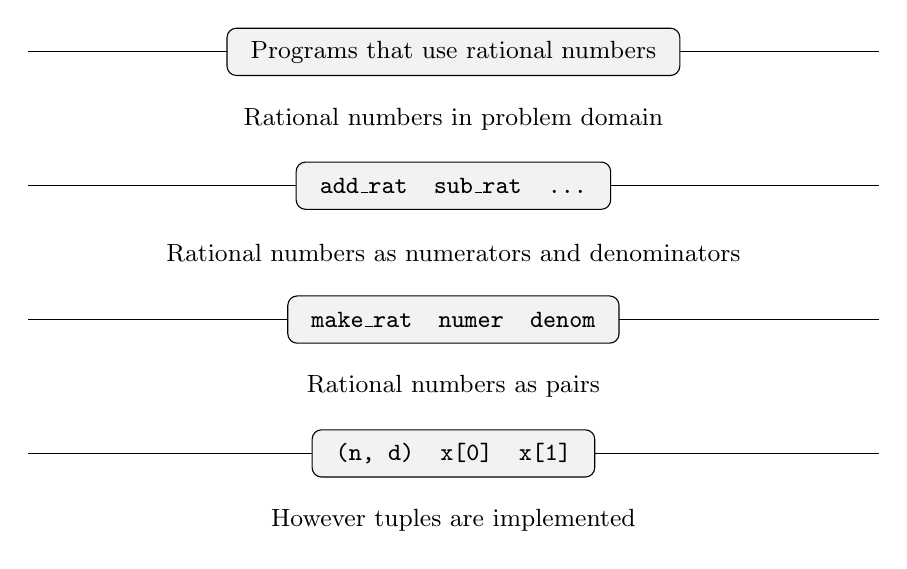
\begin{tikzpicture}[
  x = 1mm, y = 1mm,
  rule/.style = {draw, thin},
  box/.style  = {draw, thin, fill=black!5, rounded corners=1.2mm,
                 minimum height=6mm, inner xsep=3mm, font=\small},
  what/.style = {font=\small},
]

\def\halfwidth{54}

\foreach \y/\label in {%
    0/{Programs that use rational numbers},
    -17/{\ttfamily add\_rat\quad sub\_rat\quad \dots},
    -34/{\ttfamily make\_rat\quad numer\quad denom},
    -51/{\ttfamily (n, d)\quad x[0]\quad x[1]}%
  }{%
    \draw[rule] (-\halfwidth, \y) -- (\halfwidth, \y);
    \node[box] at (0, \y) {\label};
  }

\foreach \y/\label in {%
    -8.5/{Rational numbers in problem domain},
    -25.5/{Rational numbers as numerators and denominators},
    -42.5/{Rational numbers as pairs},
    -59.5/{However tuples are implemented}%
  }{%
    \node[what] at (0, \y) {\label};
  }

\end{tikzpicture}
